\documentclass[a4paper,twoside]{article}
\usepackage[T1]{fontenc}
\usepackage[bahasa]{babel}
\usepackage{color} %warna
\usepackage{graphicx}
\usepackage{graphics}
\usepackage{float}
\usepackage[cm]{fullpage}
\pagestyle{myheadings}
\usepackage{etoolbox}
\usepackage{setspace} 
\usepackage{lipsum} 
\usepackage{listings} %source code
\usepackage{lscape} %landscape untuk source code
\usepackage{multicol} %multiple column
\usepackage{ifthen} % if then
\setlength{\headsep}{30pt}
\usepackage[inner=2cm,outer=2.5cm,top=2.5cm,bottom=2cm]{geometry} %margin
% \pagestyle{empty}


\makeatletter
\renewcommand{\@maketitle} {\begin{center} {\LARGE \textbf{ \textsc{\@title}} \par} \bigskip {\large \textbf{\textsc{\@author}} }\end{center} }
\renewcommand{\thispagestyle}[1]{}
\markright{\textbf{\textsc{Laporan Perkembangan Pengerjaan Skripsi\textemdash Sem. Ganjil 2015/2016}}}

\onehalfspacing
 
\begin{document}

\title{\@judultopik}
\author{\nama \textendash \@npm} 

%ISILAH DATA DATA BERIKUT INI:
\newcommand{\nama}{Steven Sutana}
\newcommand{\@npm}{2012730046}
\newcommand{\tanggal}{25/11/2015} %Tanggal pembuatan dokumen
\newcommand{\@judultopik}{Porting PHP menjadi Play Framework (Studi Kasus : KIRI Front-End)} % Judul/topik anda
\newcommand{\kodetopik}{PAS3902}
\newcommand{\jumpemb}{1} % Jumlah pembimbing, 1 atau 2
\newcommand{\pembA}{Pascal Alfadian}
\newcommand{\pembB}{-}
\newcommand{\semesterPertama}{39 - Ganjil 15/16} % semester pertama kali topik diambil, angka 1 dimulai dari sem Ganjil 96/97
\newcommand{\lamaSkripsi}{1} % Jumlah semester untuk mengerjakan skripsi s.d. dokumen ini dibuat
\newcommand{\kulPertama}{Skripsi 1} % Kuliah dimana topik ini diambil pertama kali
\newcommand{\tipePR}{B} % tipe progress report :
% A : dokumen pendukung untuk pengambilan ke-2 di Skripsi 1
% B : dokumen untuk reviewer pada presentasi dan review Skripsi 1
% C : dokumen pendukung untuk pengambilan ke-2 di Skripsi 2
\maketitle

\pagenumbering{arabic}

\lstset{
  numbers=left,
  stepnumber=1,    
  firstnumber=1,
  numberfirstline=true
}
\lstset{basicstyle=\tiny, commentstyle=\color{blue}}
\lstset{frame=leftline, tabsize=4, breaklines=true}

\section{Data Skripsi} %TIDAK PERLU MENGUBAH BAGIAN INI !!!
Pembimbing utama/tunggal: {\bf \pembA}\\
Pembimbing pendamping: {\bf \pembB}\\
Kode Topik : {\bf \kodetopik}\\
Topik ini sudah dikerjakan selama : {\bf \lamaSkripsi} semester\\
Pengambilan pertama kali topik ini pada : Semester {\bf \semesterPertama} \\
Pengambilan pertama kali topik ini di kuliah : {\bf \kulPertama} \\
Tipe Laporan : {\bf \tipePR} -
\ifdefstring{\tipePR}{A}{
      Dokumen pendukung untuk {\BF pengambilan ke-2 di Skripsi 1} }
    {
    \ifdefstring{\tipePR}{B} {
        Dokumen untuk reviewer pada presentasi dan {\bf review Skripsi 1}}
      {  Dokumen pendukung untuk {\bf pengambilan ke-2 di Skripsi 2}}
    }

\section{Detail Perkembangan Pengerjaan Skripsi}
Detail bagian pekerjaan skripsi sesuai dengan rencan kerja/laporan perkembangan terkahir :
  \begin{enumerate}
    \item Memahami dan melakukan analisa kode KIRI yang sudah ada.\\
    {\bf status :} Ada sejak rencana kerja skripsi.\\
    {\bf hasil :} 
    Pada halaman utama KIRI (dapat dilihat pada gambar \ref{fig:3_KIRI_main}), terdapat beberapa bagian yaitu:
    \begin{enumerate}
    		\item \textbf{Peta}
    		\item \textbf{Form Samping} yang terdiri dari beberapa bagian, yaitu:
    		\begin{enumerate}
    			\item Dropdown Menu Kota
    			\item Dropdown Menu Bahasa
    			\item Textfield
    			\item Tombol Swap
    			\item Tombol Reset
    			\item Tombol Find
    		\end{enumerate}
    \end{enumerate}

\begin{figure}[H]
  \centering
  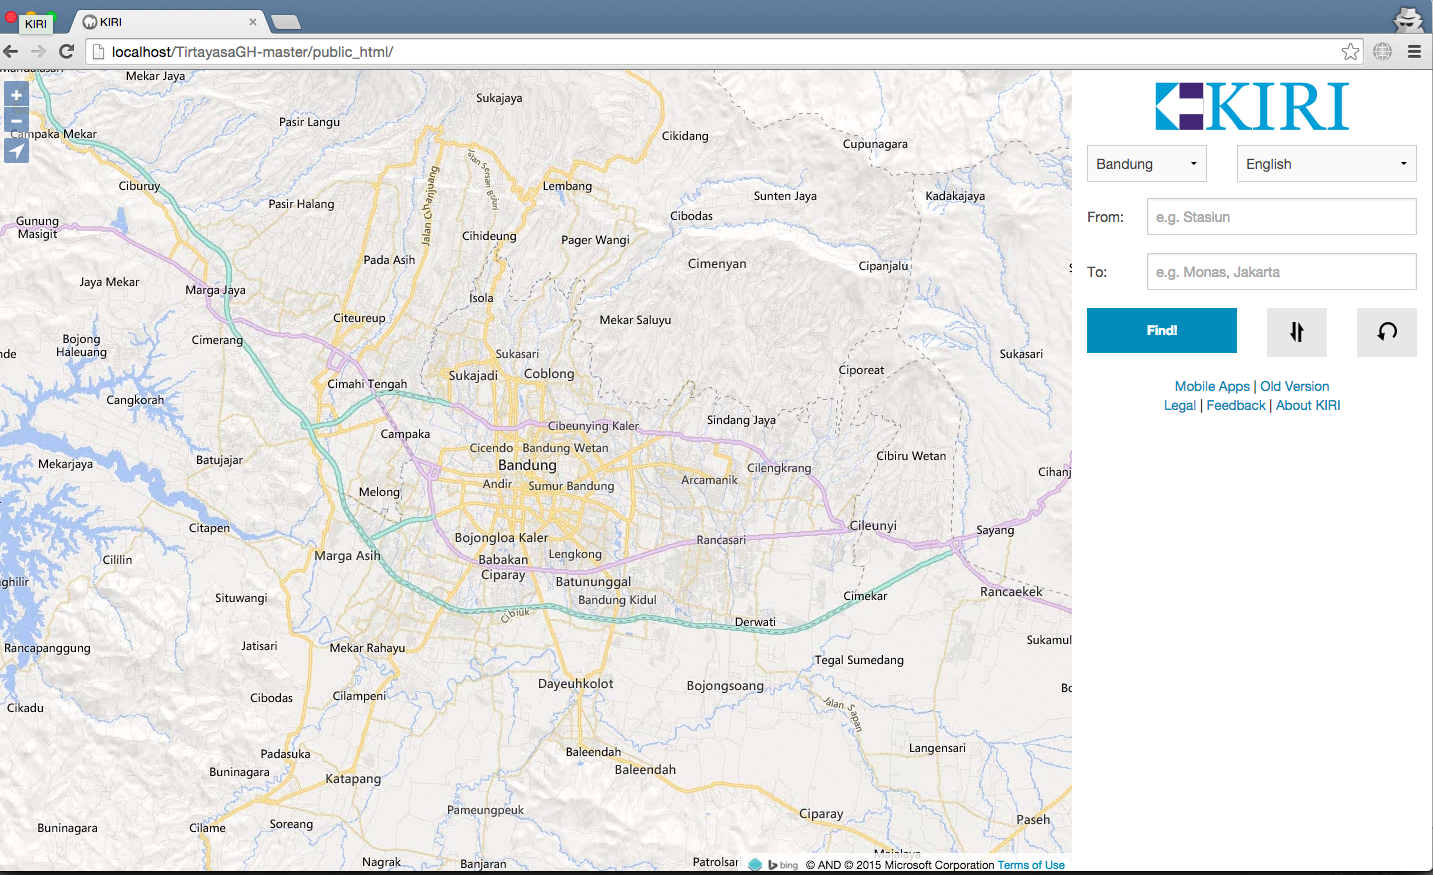
\includegraphics[scale=0.3]{Gambar/KIRI-main}
  \caption{Halaman Utama KIRI} 
  \label{fig:3_KIRI_main}
\end{figure}

\textbf{Peta}\\
Peta pada KIRI (Gambar \ref{fig:3_KIRI_peta}) berfungsi untuk menampilkan peta pada pengguna berdasarkan kota pengguna dan juga menentukan tempat asal dan tujuan pengguna dengan melakukan klik pada peta.

\begin{figure}[H]
  \centering
  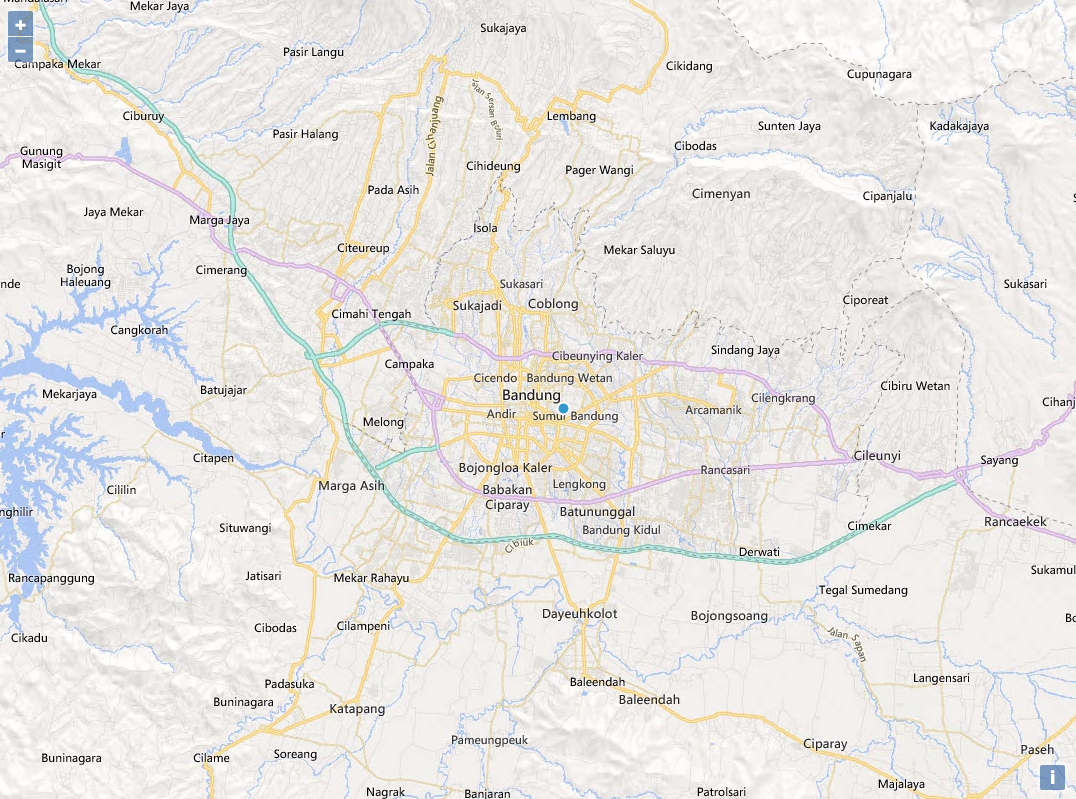
\includegraphics[scale=0.4]{Gambar/KIRI-peta}
  \caption{Peta pada KIRI} 
  \label{fig:3_KIRI_peta}
\end{figure}

KIRI menggunakan OpenLayers yang berbasis JavaScript untuk memuat peta pada halaman \textit{web}. Pertama melakukan deklarasi peta yang digunakan menggunakan BingMaps. Penggunaan BingMaps membutuhkan dua \textit{parameter}, yaitu \textit{key} yang merupakan kunci untuk menggunakan BingMaps dan \textit{imagerySet} yang merupakan tipe peta pada BingMaps. dan tipe peta pada BingMaps tersebut seperti pada kode listing \ref{lst_3_php_peta_bing}.

\begin{lstlisting}[caption=Deklarasi peta BingMaps,label = {lst_3_php_peta_bing}]
var mapLayer = new ol.layer.Tile(
{
  source : new ol.source.BingMaps(
  {
    key : 'AuV7xXD6_UMiQ5BLoZr0xkpjLpzWqMT55772Q8XtLIQeuDebHPKiNXSlZXxEr1GA',
    imagerySet : 'Road'
  })
});
\end{lstlisting}

%Untuk memunculkan tombol GPS Location yang berfungsi untuk pencarian lokasi berdasarkan lokasi pengguna. Pertama membuat elemen tombol dengan 

Untuk menambahkan fitur pada peta OpenLayers, seperti membuat marker pada peta dan membuat rute pada peta dapat dicapai dengan membuat objek ol.source.Vector seperti pada kode listing \ref{lst_3_php_peta_olvector}.

\begin{lstlisting}[caption=Objek ol.source.Vector,label = {lst_3_php_peta_olvector}]
var resultVectorSource = new ol.source.Vector();
var inputVectorSource = new ol.source.Vector();
\end{lstlisting}

Setelah deklarasi peta beserta konfigurasi fitur yang terdapat pada peta, memasukkan semua fitur pada \textit{layers} dan \textit{target} untuk memasukkan \textit{id tag} yang digunakan pada HTML seperti pada kode listing \ref{lst_3_php_peta_instansiasi}.

\begin{lstlisting}[caption=Instansiasi peta,label = {lst_3_php_peta_instansiasi}]
var map = new ol.Map(
  {
    ...
    layers : [ mapLayer, new ol.layer.Vector({source: inputVectorSource}), new ol.layer.Vector({source: resultVectorSource}) ],
    target : 'map'
});
\end{lstlisting}

\textbf{Form Samping}\\
Form yang terdapat pada halaman utama KIRI (Gambar \ref{fig:3_KIRI_form}) terdiri dari:
\begin{figure}[H]
  \centering
  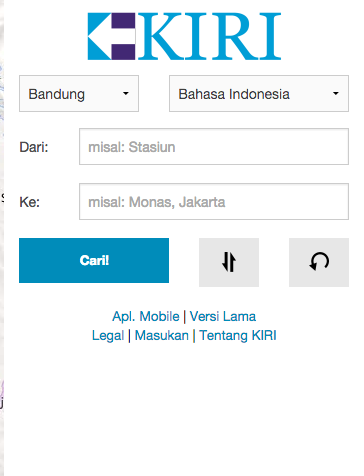
\includegraphics[scale=0.5]{Gambar/KIRI-form}
  \caption{Form pada KIRI} 
  \label{fig:3_KIRI_form}
\end{figure}

\textbf{Dropdown Menu Kota}\\
\textit{Dropdown} yang berfungsi untuk memilih kota yang akan ditampilkan pada peta (Gambar \ref{fig:3_KIRI_drop_kota}).

\begin{figure}[H]
  \centering
  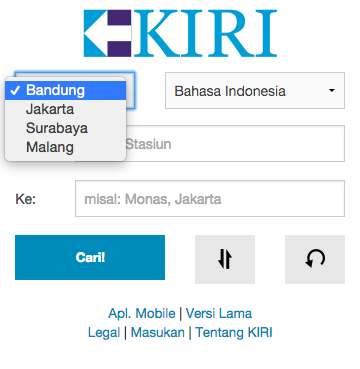
\includegraphics[scale=0.5]{Gambar/KIRI-drop-kota}
  \caption{Dropdown Menu Kota pada KIRI} 
  \label{fig:3_KIRI_drop_kota}
\end{figure}

Melakukan deklarasi variabel regioninfos sebagai \textit{associated array} pada file constants.php. Setiap kota direpresentasikan sebagai variabel proto\_region\_KOTA dimana KOTA adalah kota yang ada pada KIRI. Setiap proto\_region\_KOTA merupakan array dengan indeks:
\begin{enumerate}
	\item \textit{lat} sebagai garis lintang,
	\item \textit{lon} sebagai garis bujur,
	\item \textit{zoom} sebagai tingkat \textit{zoom} untuk memperbarui peta,
	\item \textit{name} untuk menampilkan pilihan kota,
	\item \textit{searchplace\_regex} untuk pencarian rute pada pilihan kota.
\end{enumerate} 
Kode dapat dilihat pada kode listing \ref{lst_3_php_dropdown_kota_regioninfos}.

\begin{lstlisting}[caption=Deklarasi variabel regioninfos,label = {lst_3_php_dropdown_kota_regioninfos}]
..
/** Different parameters for different regions. */
  $regioninfos = array(
    $proto_region_bandung => array(
      'lat' => -6.91474,
      'lon' => 107.60981,
      'radius' => 17000,
      'zoom' => 12,
      'searchplace_regex' => ', *(bandung|bdg)$',
      'name' => 'Bandung'
    ),
    $proto_region_jakarta => array(
      'lat' => -6.21154,
      'lon' => 106.84517,
      'radius' => 15000,
      'zoom' => 11,
      'searchplace_regex' => ', *(jakarta|jkt)$',
      'name' => 'Jakarta'
    ),
    $proto_region_surabaya => array(
      'lat' => -7.27421,
      'lon' => 112.71908,
      'radius' => 15000,
      'zoom' => 12,
      'searchplace_regex' => ', *(surabaya|sby)$',
      'name' => 'Surabaya'
    ),
    $proto_region_malang => array(
      'lat' => -7.9812985,
      'lon' => 112.6319264,
      'radius' => 15000,
      'zoom' => 13,
      'searchplace_regex' => ', *(malang|mlg)$',
      'name' => 'Malang'        
    )
  );
..
\end{lstlisting}

Untuk menampilkan pilihan kota, pertama mengambil array regioninfos, lalu melakukan pengulangan sebanyak nilai yang terdapat pada regioninfos. Dalam pengulangan tersebut, menulis \textit{tag} HTML \verb!option! sesuai dengan \textit{name} yang terdapat pada regioninfos, jika \textit{name} tersebut sama dengan \textit{region} pengguna, maka opsi tersebut akan terpilih. Kode dapat dilihat pada kode listing \ref{lst_3_php_dropdown_kota_tampilan}

\begin{lstlisting}[caption=Menampilkan pilihan kota kepada pengguna ,label = {lst_3_php_dropdown_kota_tampilan}]
..
<select class="fullwidth" id="regionselect">
  <?php
    foreach ($regioninfos as $key => $value) {
      print "<option value=\"$key\"";
      if ($key == $region) {
        print " selected";
      }
      print ">" . $value['name'] . "</option>\n";
    }
  ?>
</select>
..
\end{lstlisting}

Untuk memperbarui peta, KIRI menggunakan fungsi JavaScript dengan menerima dua parameter, yaitu newRegion dan updateCookie. Pertama membuat \textit{cookie} dengan kunci region, lalu membuat variabel \textit{point} dengan mengubah String menjadi LonLat dari titik tengah peta yang dituju. Untuk memperbarui peta dengan mengatur titik tengah pada peta yaitu memanggil \textit{method} \verb!setCenter! yang menerima parameter ol.proj.transform yang berisi garis lintang dan bujur serta kode dari Sistem  dan Transformasi  Koordinat. Setelah itu, mengatur tingkat \textit{zoom} dengan memanggil \textit{method} \verb!setZoom! dengan parameter berupa tingkat \textit{zoom} dari peta yang dituju. Kode dapat dilihat pada kode listing \ref{lst_3_php_dropdown_kota_update}

\begin{lstlisting}[caption=Fungsi JavaScript untuk memperbarui peta ,label = {lst_3_php_dropdown_kota_update}]
/**
 * Updates the region information in this page.
 */
function updateRegion(newRegion, updateCookie) {
  region = newRegion;
  setCookie('region', region);
  var point = stringToLonLat(regions[region].center);
  map.getView().setCenter(ol.proj.transform(point, 'EPSG:4326', 'EPSG:3857'));
  map.getView().setZoom(regions[region].zoom);
}
\end{lstlisting}

Untuk melakukan pengubahan dari tipe data String menjadi \textit{array} Float yang berguna menjadi garis lintang dan garis bujur dengan cara memanggil \textit{method} \verb!split! dengan \textit{parameter} `,` yang berfungsi membuang `,` dan menjadikan \textit{array}. Setelah menjadi \textit{array}, String tersebut masing-masing dijadikan ke tipe data Float dengan cara memanggil \textit{method} \verb!parseFloat! dengan \textit{parameter} String yang ingin dijadikan Float. Kode dapat dilihat pada kode listing \ref{lst_3_php_dropdown_kota_parse}.

\begin{lstlisting}[caption=Fungsi JavaScript untuk mengubah String menjadi \textit{array} Float ,label = {lst_3_php_dropdown_kota_parse}]
/**
 * Converts "lat,lng" into lonlat array
 * @return the converted lonlat array
 */
function stringToLonLat(text) {
  var latlon = text.split(/,\s*/);
  return [parseFloat(latlon[1]), parseFloat(latlon[0])];
}
\end{lstlisting}

\textbf{Dropdown Menu Bahasa}\\
\textit{Dropdown} yang berfungsi untuk memilih bahasa yang akan digunakan pada KIRI (Gambar \ref{fig:3_KIRI_drop_bahasa}).

\begin{figure}[H]
  \centering
  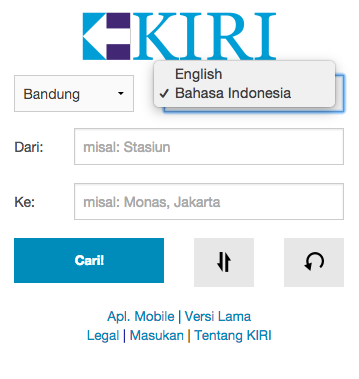
\includegraphics[scale=0.5]{Gambar/KIRI-drop-bahasa}
  \caption{Dropdown Menu Bahasa pada KIRI} 
  \label{fig:3_KIRI_drop_bahasa}
\end{figure}

Untuk menampilkan pilihan bahasa, menggunakan \textit{tag} HTML \verb!option!. Pada bagian ini, hanya cek jika sudah dilakukan lokalisasi ke Bahasa Indonesia, maka opsi yang terpilih adalah Bahasa Indonesia. Kode dapat dilihat pada \ref{lst_3_php_dropdown_bahasa_tampilan}

\begin{lstlisting}[caption=Menampilkan pilihan bahasa kepada pengguna ,label = {lst_3_php_dropdown_bahasa_tampilan}]
..
<select class="fullwidth" id="localeselect">
  <option value="en">English</option>
  <option value="id"
    <?php if ($locale == $proto_locale_indonesia) print " selected"; ?>>Bahasa
    Indonesia</option>
</select>
..
\end{lstlisting}

Ketika memilih \textit{dropdown} bahasa, memanggil \textit{method} JavaScript dengan \textit{parameter} berupa fungsi yang berisi menambahkan URL dengan \textit{query} \verb!locale=id! atau \verb!locale=en!. Kode dapat dilihat pada kode listing \ref{lst_3_php_dropdown_bahasa_fungsi}.

\begin{lstlisting}[caption=Fungsi JavaScript untuk Internationalization ,label = {lst_3_php_dropdown_bahasa_fungsi}]
..
// Event handlers
var localeSelect = $('#localeselect');
localeSelect.change(function() {
  // IE fix: when window.location.origin is not available 
  if (!window.location.origin) {
    window.location.origin = window.location.protocol + "//" + window.location.hostname + (window.location.port ? ':' + window.location.port: '');
  }
  window.location.replace(window.location.origin + "?locale=" + localeSelect.val());
});
..
\end{lstlisting}


\textbf{Textfield}\\
\textit{Textfield} pada KIRI menggunakan PHP agar dapat dilakukan proses Internationalization, seperti pada kode listing \ref{lst_3_php_textfield_from} untuk \textit{textfield} tempat asal dan kode listing \ref{lst_3_php_textfield_to} untuk \textit{textfield} tempat tujuan. Textfield pada KIRI dapat menerima dua masukan pengguna, yaitu:

\begin{lstlisting}[caption=Menampilkan \textit{textfield} tempat awal kepada pengguna ,label = {lst_3_php_textfield_from}]
..
<div class="small-2 columns">
  <label for="startInput" class="inline"><?php print $index_from; ?></label>
</div>
<div class="small-10 columns">
  <input type="text" id="startInput" value=""
    placeholder="<?php print $index_placeholder_start; ?>">
</div>
..
\end{lstlisting}

\begin{lstlisting}[caption=Menampilkan \textit{textfield} tempat tujuan kepada pengguna ,label = {lst_3_php_textfield_to}]
..
<div class="small-2 columns">
  <label for="finishInput" class="inline"><?php print $index_to; ?></label>
</div>
<div class="small-10 columns">
  <input type="text" id="finishInput" value=""
    placeholder="<?php print $index_placeholder_finish; ?>">
</div>
..
\end{lstlisting}

\begin{enumerate}
  \item \textbf{Textfield dengan Masukan Nama Tempat}, pengguna dapat memasukkan nama tempat asal dan tujuan (Gambar \ref{fig:3_KIRI_textfield_nama})
  
  \begin{figure}[H]
    \centering
    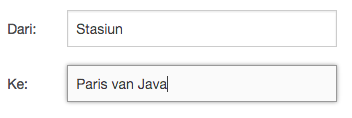
\includegraphics[scale=0.5]{Gambar/KIRI-textfield-nama}
    \caption{Input User(Nama Tempat)} 
    \label{fig:3_KIRI_textfield_nama}
  \end{figure}
  
  \item \textbf{Textfield dengan Masukan Klik Peta}, pengguna memasukkan koordinat tempat asal dan tujuan dengan klik pada peta. Dengan melakukan klik pada peta, textfield tempat asal dan tujuan akan akan secara otomatis terisi oleh koordinat masing-masing tempat (Gambar \ref{fig:3_KIRI_textfield_koord}).
  
  \begin{figure}[H]
    \centering
    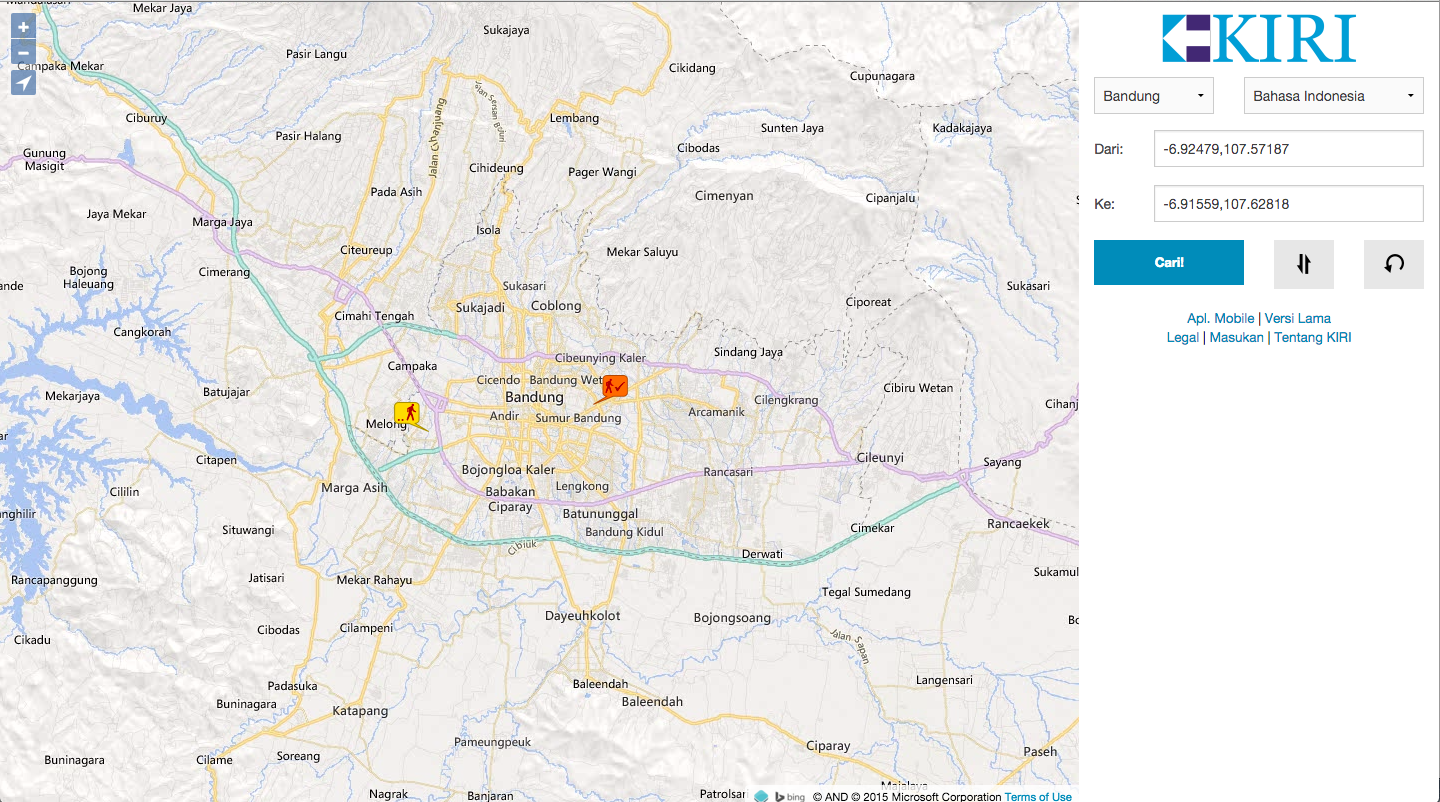
\includegraphics[scale=0.3]{Gambar/KIRI-textfield-koord}
    \caption{Input User(Klik pada peta)} 
    \label{fig:3_KIRI_textfield_koord}
  \end{figure}
  
  Agar peta dapat diklik, maka memanggil method \verb!on! dengan parameter `click` dan fungsi yang akan diimplementasikan ketika melakukan klik pada peta. Isi fungsi tersebut adalah pertama melakukan pengecekan apabila textfield tempat asal atau tempat tujuan kosong, maka membuat geometry yang merupakan objeck ol.geom.Point dengan parameter koordinat pada peta yang diklik oleh pengguna, lalu membuat marker dengan gambar start.png bila textfield tempat asal kosong atau finish.png bila textfield tempat tujuan kosong. Setelah itu, menambahkan fitur marker ke inputVectorSource yang akan ditampilkan pada peta dan menulis koordinat pada textfield tempat asal atau tempat tujuan. Kode dapat dilihat pada kode listing \ref{lst_3_php_textfield_koord_kode}.
  
  \begin{lstlisting}[caption=Membuat \textit{event} klik pada peta,label = {lst_3_php_textfield_koord_kode}]
..
// Map click event
map.on('click', function(event) {
      if ($('#startInput').val() === '') {
    markers['start'] = new ol.Feature({
      geometry: new ol.geom.Point(event.coordinate)
    })
    markers['start'].setStyle(new ol.style.Style({
      image: new ol.style.Icon({
        src: 'images/start.png',
        anchor: [1.0, 1.0]
      })
    }));
    inputVectorSource.addFeature(markers['start']);
        $('#startInput').val(latLngToString(ol.proj.transform(event.coordinate, 'EPSG:3857', 'EPSG:4326')));
      } else if ($('#finishInput').val() === '') {
    markers['finish'] = new ol.Feature({
      geometry: new ol.geom.Point(event.coordinate)
    })
    markers['finish'].setStyle(new ol.style.Style({
      image: new ol.style.Icon({
        src: 'images/finish.png',
        anchor: [0.0, 1.0]
      })
    }));
    inputVectorSource.addFeature(markers['finish']);
        $('#finishInput').val(latLngToString(ol.proj.transform(event.coordinate, 'EPSG:3857', 'EPSG:4326')));
      }
});
..
\end{lstlisting}

\end{enumerate}

\textbf{Tombol Swap}\\
Pengguna dapat menukar isi dari \textit{textfield} tempat asal dan tujuan. Pertama kali yang dilakukan adalah mencari pada dokumen dengan \textit{id} swapbutton dan memanggil \textit{method} \verb!click! dengan \textit{parameter} fungsi swapInput seperti pada kode listing \ref{lst_3_php_swap}. Fungsi swapInput berisi melakukan pencarian pada dokumen dengan id startInput dan finishInput. Melakukan penampungan sementara dengan mengambil isi dari textfield tempat asal, lalu mengubah isi dari textfield tempat asal dengan tujuan dan mengubah isi dari textfield tempat tujuan dengan isi dari penampungan sementara. Setelah itu, jika kedua textfield ada isinya, melakukan pencarian rute. Kode dapat diliihat pada kode listing \ref{lst_3_php_swap_fungsi}.

\begin{lstlisting}[caption=\textit{Method} untuk memanggil fungsi JavaScript ketika tombol \textit{swap} ditekan ,label = {lst_3_php_swap}]
..
$('#swapbutton').click(swapInput);
..
\end{lstlisting}

\begin{lstlisting}[caption=Fungsi JavaScript untuk menukar isi \textit{textfield} tempat asal dan tujuan ,label = {lst_3_php_swap_fungsi}]  
/**
 * Swap the inputs
 */
function swapInput() {
  var startInput = $('#startInput');
  var finishInput = $('#finishInput');
  var temp = startInput.val();
  startInput.val(finishInput.val());
  finishInput.val(temp);
  coordinates['start'] = null;
  coordinates['finish'] = null;
  if (startInput.val() != '' && finishInput.val() != '') {
    findRouteClicked();
  }
}
\end{lstlisting}

\textbf{Tombol Reset}\\
Pengguna dapat melakukan pemilihan tempat dari awal dan mengulang tampilan peta. Pertama kali yang dilakukan adalah mencari pada dokumen dengan \textit{id} resetbutton dan memanggil \textit{method} \verb!click! dengan \textit{parameter} fungsi resetScreen seperti pada kode listing \ref{lst_3_php_reset}. 

\begin{lstlisting}[caption=\textit{Method} untuk memanggil fungsi JavaScript ketika tombol \textit{reset} ditekan ,label = {lst_3_php_reset}]
..
$('#resetbutton').click(resetScreen);
..
\end{lstlisting}

Fungsi resetScreen berisi berbagai fungsi seperti pada kode listing \ref{lst_3_php_reset_fungsi}, yaitu:

\begin{lstlisting}[caption=Fungsi JavaScript resetScreen ,label = {lst_3_php_reset_fungsi}]  
function resetScreen() {
  clearRoutingResultsOnTable();
  clearRoutingResultsOnMap();
  clearAlerts();
  clearStartFinishMarker();
  $.each(['start', 'finish'], function(sfIndex, sfValue) {
    var placeInput = $('#' + sfValue + 'Input');
    placeInput.val('');  
    placeInput.prop('disabled', false);
    $('#' + sfValue + 'Select').addClass('hidden');
  });
}
\end{lstlisting}

\begin{enumerate}
  \item \textbf{Fungsi clearRoutingResultsOnMap}\\
  Fungsi untuk menghapus pada resultVectorSource yang merupakan berbagai \textit{marker} pada peta sebagai hasil pencarian rute dan memperbarui peta. Kode dapat dilihat pada kode listing \ref{lst_3_php_reset_clearMap}.
  \begin{lstlisting}[caption=Fungsi JavaScript untuk menghapus hasil pencarian rute pada peta ,label = {lst_3_php_reset_clearMap}]
  function clearRoutingResultsOnMap() {
    resultVectorSource.clear();
    updateRegion(region, false);
  }
  \end{lstlisting}
  
  \item \textbf{Fungsi clearRoutingResultsOnTable}\\
  Fungsi untuk menghapus tampilan tabel sebagai hasil pencarian rute yang akan ditampilkan pada pengguna. Kode dapat dilihat pada kode listing \ref{lst_3_php_reset_clearTable}.
  
  \begin{lstlisting}[caption=Fungsi JavaScript untuk menghapus tampilan tabel,label = {lst_3_php_reset_clearTable}]
  function clearRoutingResultsOnTable() {
    $('.tabs').remove();
    $('.tabs-content').remove();
  }
  \end{lstlisting}
  
  \item \textbf{Fungsi clearAlerts}\\
  Fungsi untuk menghapus \textit{alerts} sebagai tanda yang akan ditampilkan kepada pengguna, seperti sedang melakukan pencarian rute atau masalah koneksi. Kode dapat dilihat pada kode listing \ref{lst_3_php_reset_clearAlerts}.
  
  \begin{lstlisting}[caption=Fungsi JavaScript untuk menghilangkan \textit{alerts},label = {lst_3_php_reset_clearAlerts}]
  function clearAlerts() {
    $('.alert-box').remove();
  }
  \end{lstlisting}
  
  \item \textbf{Fungsi clearRoutingResultsOnMap}\\
  Fungsi untuk menghapus \textit{markers} tempat awal dan tujuan, lalu menghapus fitur pada inputVectorSource. Kode dapat dilihat pada kode listing \ref{lst_3_php_reset_clearMarker}.
  
  \begin{lstlisting}[caption=Fungsi JavaScript untuk menghilangkan \textit{alerts},label = {lst_3_php_reset_clearMarker}]
  function clearStartFinishMarker() {
    if (markers['start'] != null) {
      markers['start'] = null;
    }
    if (markers['finish'] != null) {
      markers['finish'] = null;
    }
    inputVectorSource.clear();
  }
  \end{lstlisting}
  
\end{enumerate}

\textbf{Tombol Find}\\
Pengguna dapat mencari rute untuk sampai ke tujuan (Gambar \ref{fig:3_KIRI_find}). Pengguna dapat memilih rute alternatif yang sudah disediakan KIRI jika ada (Gambar \ref{fig:3_KIRI_find_alternate}).

\begin{figure}[H]
  \centering
  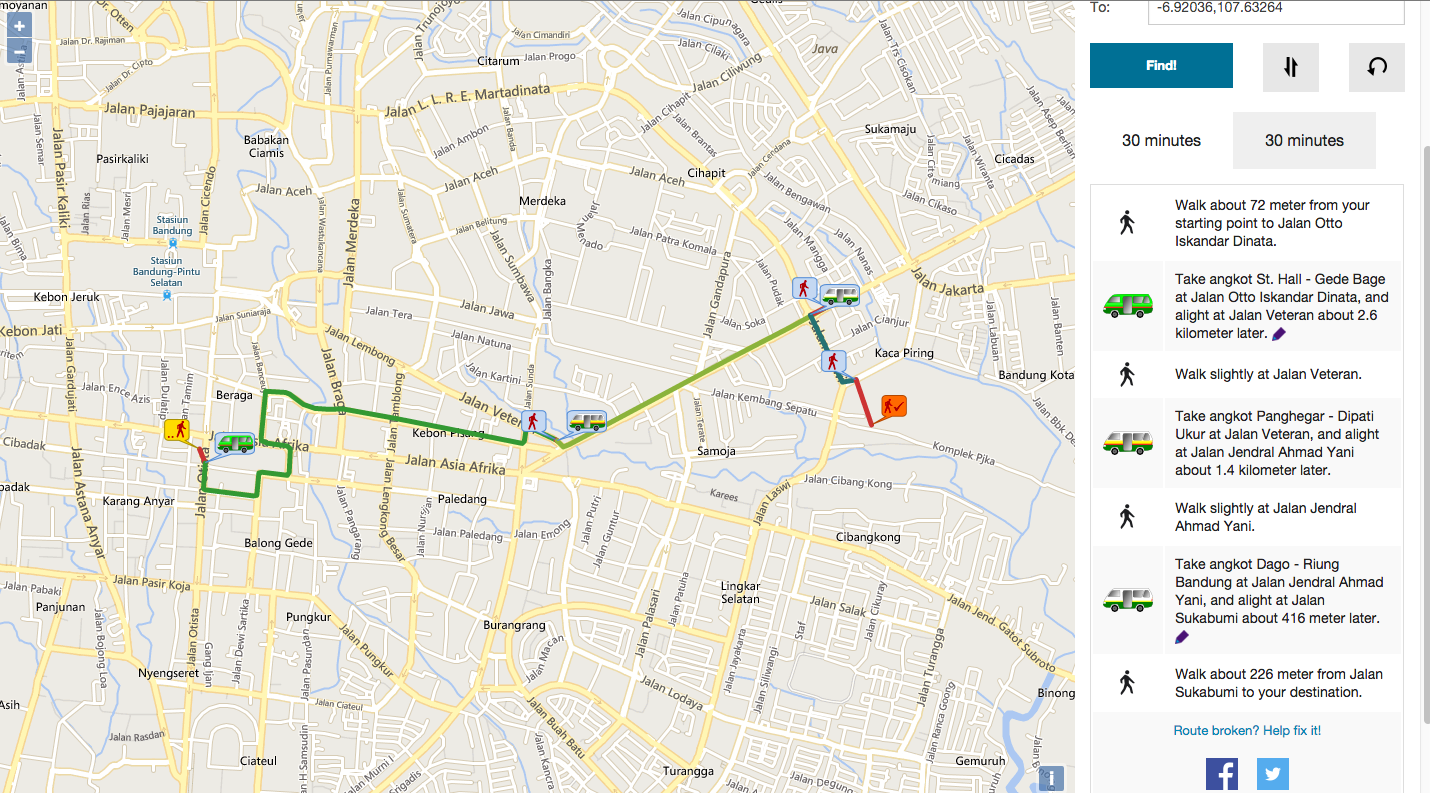
\includegraphics[scale=0.3]{Gambar/KIRI-find}
  \caption{Contoh Pencarian Rute pada KIRI} 
  \label{fig:3_KIRI_find}
\end{figure}

\begin{figure}[H]
  \centering
  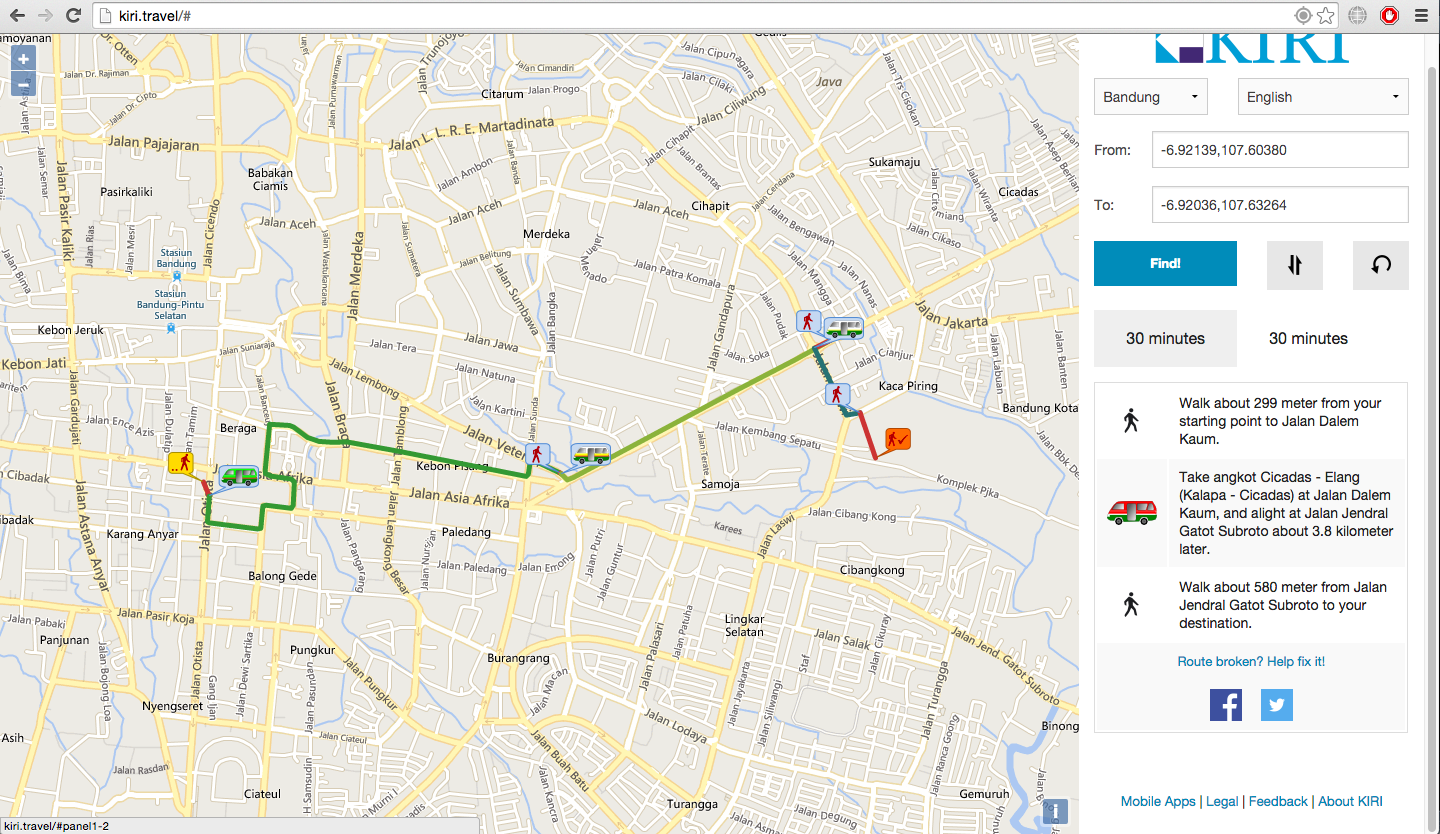
\includegraphics[scale=0.3]{Gambar/KIRI-find-alternate}
  \caption{Contoh Rute Alternatif pada KIRI} 
  \label{fig:3_KIRI_find_alternate}
\end{figure}

Hal yang pertama kali dilakukan adalah melakukan validasi jika salah satu textfield kosong, maka akan langsung membatalkan proses dan memberi alert kepada pengguna. Jika tidak kosong, maka akan memunculkan alert `mohon menunggu`. 
Setelah itu melakukan pengecekan apakah isi dari textfield merupakan format yang bener untuk garis lintang dan bujur. Jika formatnya benar, maka dimasukkan ke dalam array coordinates dan melakukan penambahan completedLatLon yang berfungsi untuk mengetahui apakah kedua textfield sudah benar formatnya untuk dilakukan pencarian rute. Jika formatnya tidak benar, maka melakukan pengecekan array coordinates kosong atau tidak. 
Jika kosong, maka melakukan pencarian pilihan tempat yang akan menjadi tempat sugesti yang diberikan kepada pengguna. Jika tidak kosong, maka memanggil fungsi checkCoordinatesThenRoute dengan parameter berupa coordinates. Terakhir, melakukan pengecekan completedLatLon jika isinya sama dengan dua, maka memanggil fungsi checkCoordinatesThenRoute. Kode dapat dilihat pada kode listing \ref{lst_3_php_find_fungsi}.

\begin{lstlisting}[caption=Fungsi JavaScript untuk ketika tombol \textit{find} ditekan,label = {lst_3_php_find_fungsi}]
/**
 * A function that will be called when find route button is clicked
 * (or triggered by another means)
 */
function findRouteClicked() {
  // Validate
  var cancel = false;
  $.each(['start', 'finish'], function(sfIndex, sfValue) {
    if ($('#' + sfValue + 'Input').val() === '') {
      cancel = true;    
      return;
    }
  });
  if (cancel) {
    showAlert(messageFillBoth, 'alert');      
    return;
  }
  
  clearAlerts();
  clearRoutingResultsOnTable();
  showAlert(messagePleaseWait, 'secondary');
  
  var completedLatLon = 0;
  $.each(['start', 'finish'], function(sfIndex, sfValue) {
    var placeInput = $('#' + sfValue + 'Input');
    var placeSelect = $('#' + sfValue + 'Select');
    if (isLatLng(placeInput.val())) {
      coordinates[sfValue] = placeInput.val();
      completedLatLon++;
    } else {
      if (coordinates[sfValue] == null) {
        // Coordinates not yet ready, we do a search place
        protocol.searchPlace(
            placeInput.val(),
            region,
            function(result) {
              placeSelect.empty();
              placeSelect.addClass('hidden');
              if (result.status != 'error') {
                if (result.searchresult.length > 0) {
                  $.each(result.searchresult, function(index, value) {
                    var placeSelect = $('#' + sfValue + 'Select');
                    placeSelect
                           .append($('<option></option>')
                           .attr('value',value['location'])
                           .text(value['placename']));
                    placeSelect.removeClass('hidden');
                  });
                  coordinates[sfValue] = result.searchresult[0]['location'];
                  checkCoordinatesThenRoute(coordinates);
                } else {
                  clearSecondaryAlerts();
                  clearRoutingResultsOnMap();
                  showAlert(placeInput.val() + messageNotFound, 'alert');
                }
              } else {
                clearSecondaryAlerts();
                clearRoutingResultsOnMap();
                showAlert(messageConnectionError, 'alert');
              }
            });
      } else {
        // Coordinates are already available, skip searching
        checkCoordinatesThenRoute(coordinates);
      }
    }
  });
  if (completedLatLon == 2) {
    checkCoordinatesThenRoute(coordinates);
  }
}
\end{lstlisting}

Fungsi checkCoordinatesThenRoute melakukan pengecekan jika array coordinates tempat awal dan tempat tujuan tidak kosong maka melakukan protocol.findRoute. Jika hasil results sama dengan `ok`, maka menunjukkan rute pencarian. Jika hasil result bukan `ok`, maka akan menampilkan alert `gangguan koneksi`. Kode dapat dilihat pada kode listing \ref{lst_3_php_find_checkRoute}.
\begin{lstlisting}[caption=Fungsi JavaScript checkCoordinatesThenRoute,label = {lst_3_php_find_checkRoute}]
/**
 * Check if coordinates are complete. If yes, then start routing.
 * @param coordinates the coordinates to check.
 */
function checkCoordinatesThenRoute(coordinates) {
  if (coordinates['start'] != null && coordinates['finish'] != null) {
    protocol.findRoute(
        coordinates['start'],
        coordinates['finish'],
        locale,
        function(results) {
          if (results.status === 'ok') {
            showRoutingResults(results);
          } else {
            clearSecondaryAlerts();
            showAlert(messageConnectionError, 'alert');
          }
        });
  }
}
\end{lstlisting}

\textbf{Internationalization}\\
Penggunaan Internationalization (i18n) pada PHP dengan cara deklarasi semua variabel yang akan digunakan pada proses i18n terlebih dahulu, misalnya buat file dengan nama tirtayasa\_en.php untuk Bahasa Inggris dan tirtayasa\_id.php untuk Bahasa Indonesia. Pada setiap file tersebut, masukkan \textit{script} PHP untuk menentukan teks yang keluar pada halaman \textit{web} seperti pada kode listing \ref{lst_3_i18n_en} dan kode listing \ref{lst_3_i18n_id}. 

\begin{lstlisting}[caption=Script PHP untuk Bahasa Inggris,label = {lst_3_i18n_en}]
<?php

  $index_about_kiri = "About KIRI";
  $index_apps = "Mobile Apps";
  $index_advanced_ = "Advanced...";
  $index_buyticket = "BUY TICKET";
  $index_connectionerror = 'Connection problem';
?>
\end{lstlisting}


\begin{lstlisting}[caption=Script PHP untuk Bahasa Indonesia,label = {lst_3_i18n_id}]
<?php
  $index_about_kiri = "Tentang KIRI";
  $index_apps = "Apl. Mobile";
  $index_advanced_ = "Lanjut...";
  $index_buyticket = "BUY TICKET";
  $index_connectionerror = 'Gangguan koneksi';
?>
\end{lstlisting}

Setelah itu, masukkan \textit{script} PHP pada \textit{tag} HTML yang ingin diubah saat dilakukan i18n. Adanya \textit{script} PHP pada tag HTML, maka teks akan berubah jika dilakukan i18n seperti pada kode listing \ref{lst_3_i18n_php}.

\begin{lstlisting}[caption=Script PHP untuk Internationalization,label = {lst_3_i18n_php}]
  ...
  <label for="startInput" class="inline"><?php print $index_from; ?></label>
  <label for="finishInput" class="inline"><?php print $index_to; ?></label>
  <a href="#" class="small button expand" id="findbutton"><strong><?php print $index_find; ?></strong></a>
  ...
\end{lstlisting}
    
    
    \item Melakukan studi literatur tentang metode yang berkaitan dengan kode PHP dan Java (Play Framework).\\
    {\bf status :} Ada sejak rencana kerja skripsi.\\
    {\bf hasil :}
    
\textbf{Play Framework}\\
Play Framework \cite{playforjava} merupakan \textit{framework} untuk aplikasi web dengan menggunakan bahasa Java dan Scala. Play Framework tidak sepenuhnya menggunakan bahasa Java, tetapi ada juga bahasa Scala. Terdapat bahasa Scala bukan berarti harus mempelajari bahasa Scala karena dalam Play 2 dilengkapi dengan Java API yang komplit, memberikan opsi untuk memilih bahasa pemrograman yang cocok. Play Framework mempunyai antarmuka yang sederhana, nyaman, fleksibel, dan kuat. Referensi yang digunakan membahas Play Framework 2.2, sedangkan versi Play Framework yang dipakai dalam penelitian ini adalah versi 2.4. Ada sedikit perbedaan sintaks yang akan dijelaskan pada bagian yang berbeda.
Beberapa fitur utama yang membuat Play Framework produktif dan penggunaan yang nyaman:

\begin{enumerate}
  \item Penggunaan Play Framework sederhana.
  \item Konfigurasi skema URL aplikasi deklaratif.
  \item Pemetaan type-safety.
  \item Play Framework menyediakan contoh sintaks type-safety.
  \item Arsitektur yang mencakup teknologi HTML5.
  \item Kode langsung aktif berubah ketika memuat kembali halaman web.
  \item Fitur \textit{full-stack web-framework}, termasuk \textit{persistence}, keamanan, dan \textit{internationalization}. \textit{Persistence} adalah ide yang menggunakan koneksi TCP yang sama untuk mengirim dan menerima beberapa HTTP \textit{requests/responses} tanpa membuka TCP baru untuk setiap \textit{requests/responses} dengan tujuan untuk meningkatkan kinerja HTTP.
  \item Mendukung aplikasi \textit{event-driven} dan dinamis.
\end{enumerate}

Play Framework memiliki struktur yang dapat dilihat pada gambar \ref{fig:2_play_struktur}.

\begin{figure}[H]
  \centering
  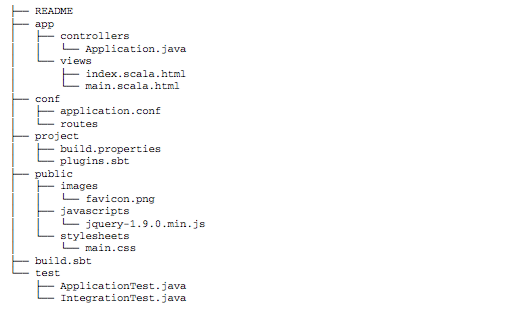
\includegraphics[scale=0.7]{Gambar/play-struktur}
  \caption{Struktur Play Framework} 
  \label{fig:2_play_struktur}
\end{figure}

\textbf{Direktori conf.}\\
Konfigurasi Play Framework terdapat pada direktori \textit{conf}. Dalam direktori \textit{conf}, terdapat file \textit{application.conf} dan \textit{routes}. File \textit{application.conf} mengandung informasi data konfigurasi aplikasi, seperti \textit{logging}, koneksi basis data, dan port berapa server berjalan. File \textit{routes} menentukan \textit{routes} aplikasi, yaitu pemetaan dari URL HTTP ke kode aplikasi. Setiap \textit{routes} memiiki tiga bagian, yaitu HTTP \textit{method}, URL \textit{path}, dan \textit{action method}. HTTP \textit{method} merupakan metode yang dipakai dalam pengiriman HTTP. URL \textit{path} adalah URL yang dipakai untuk mengakses halaman. \textit{Action method} merupakan metode  yang dipanggil ketika mengakses halaman pada URL \textit{path}. Sebagai contoh dapat dilihat pada \ref{fig:2_play_routes}, HTTP \textit{method} yang dipakai pada URL /list adalah HTTP \textit{method} GET dan akan memanggil \textit{method} list pada kelas Products di controllers.

\begin{figure}[H]
  \centering
  
\includegraphics[scale=0.7]{Gambar/play-routes}
  \caption{Contoh \textit{Routes}} 
  \label{fig:2_play_routes}
\end{figure}

\textbf{Direktori public}\\
Direktori \textit{public} mengandung semua sumber daya yang disediakan langsung tanpa melalui proses terlebih dahulu. Direktori \textit{public} biasanya mengandung file gambar, \textit{stylesheets}, JavaScript, dan halaman statis HTML. Contoh direktori \textit{public} dapat dilihat pada gambar \ref{fig:2_play_struktur}.
%
%\begin{figure}[H]
%  \centering
%  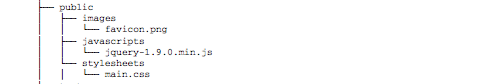
\includegraphics{Gambar/play-public}
%  \caption{Contoh Direktori \textit{public}} 
%  \label{fig:2_play_public}
%\end{figure}

\textbf{Direktori app.}\\
Direktori \textit{app} merupakan direktori utama pada aplikasi. Direktori \textit{app} berisi kode aplikasi dan berbagai kebutuhan untuk menyusun aplikasi, seperti sumber file Java dan file \textit{template}. Contoh direktori \textit{app} pada saat pertama kali membuat aplikasi Play dapat dilihat pada gambar \ref{fig:2_play_struktur}. 

Dalam \textit{controller}, terdapat file Application.java yang berisi kode Java untuk memuat halaman \textit{view}. \textit{Controller} adalah kelas untuk menerima HTTP \textit{request} dan mengembalikan nilai dari HTTP \textit{request} berupa view. Ada dua file template, yaitu index.scala.html dan main.scala.html yang berfungsi untuk menentukan halaman HTML yang akan dimuat. Semua konten yang dihasilkan di server dan dikirimkan ke klien seperti halaman HTML disebut \textit{view}. View dapat menerima parameter yang didefinisikan pada template view. Contoh view dengan menerima parameter berupa String dapat dilihat pada kode listing \ref{lst_2_view}. \textit{Method} pada \textit{Controller} menghasilkan hasil berupa \textit{Result} yang berupa \textit{view} dengan memberi parameter "Hello World". \textit{Method} pada \textit{controller} dan \textit{view} dihubungkan melalui pendefinisian pada \textit{routes}. Sebagai contoh pada kode listing \ref{lst_2_controller}, \textit{method ok} membangun HTTP \textit{response} yang mengandung \textit{response body} sebagai hasil dari \textit{template list}. \textit{Method ok} menerima \textit{parameter} berupa "Hello World". Pada \cite{playforjava}, hasil Result dalam \verb!static!, tetapi pada Play Framework 2.4 \verb!static! dihilangkan.

\begin{lstlisting}[caption=Contoh View,label = {lst_2_view},language=Java]
@(title: String)

  <!DOCTYPE html>

  <html>
         <head>
          <title>@title</title>
          <link rel="stylesheet" media="screen" href="@routes.Assets.at("stylesheets/main.css")">
          <link rel="shortcut icon" type="image/png" href="@routes.Assets.at("images/favicon.png")">
          <script src="@routes.Assets.at("javascripts/jquery-1.9.0.min.js")" type="text/javascript"></script>
        </head>
        <body>
            @title
        </body>
  </html>
\end{lstlisting}


\begin{lstlisting}[caption=Contoh Controller,label = {lst_2_controller},language=Java]
  public Result index() {
        return ok(index.render("Hello World"));
    }
\end{lstlisting}

Beberapa alternatif hasil Results, yaitu:
\begin{enumerate}
  \item \textbf{Method ok} \\
  Method yang berfungsi untuk mengembalikan Result dengan kode \textit{HTTP Response} 200 atau sukses dalam mengirim \textbf{HTTP Request}.
  \item \textbf{Method notFound} \\
  Method yang berfungsi untuk mengembalikan Result dengan  kode \textit{HTTP Response} 404 atau tidak ada halaman yang dituju.
  \item \textbf{Method badRequest} \\
  Method yang berfungsi untuk mengembalikan Result dengan kode \textit{HTTP Response} 400 atau adanya kesalahan masukan pengguna.
  \item \textbf{Method internalServerError}\\
  Method yang berfungsi untuk mengembalikan Result dengan kode \textit{HTTP Response} 500 atau adanya kesalahan pada server.
  \item \textbf{Method status}\\
  Method yang berfungsi untuk mengembalikan Result dengan kode \textit{HTTP Response} yang dapat ditentukan sendiri beserta pesannya.
  \item \textbf{Method redirect}\\
  Method yang berfungsi untuk mengembalikan Result untuk mengalihkan halaman.
\end{enumerate}

\textbf{Body Parsers}\\
\textit{Body parsers} bertugas untuk melakukan pemetaan \textit{request body} menjadi objek. Setiap \textit{action method} POST dan PUT mengandung \textit{body}. Jumlah \textit{body} dapat satu atau banyak, dan dapat berupa XML, JSON, data biner, atau dapat berupa apapun sesuai Content-Type pada \textit{header request}. \textit{Body parsers} akan menguraikan \textit{body} menjadi objek Java. \textit{Body parsers} mengubah \textit{request} menjadi objek yang dapat digunakan oleh komponen Play. Karena \textit{body} JSON dan \textit{body} XML berbeda penguraiannya, Play menggunakan \textit{body parsers} yang berbeda pula implementasinya. Berbeda Content-Type pada \textit{header request}, \textit{body parsers} spesifik dapat mengubah data yang masuk menjadi sesuatu yang dapat dimengerti oleh Play. Ilustrasi dapat dilihat pada gambar \ref{fig:2_play_bodyparsers}.

\begin{figure}[H]
  \centering
  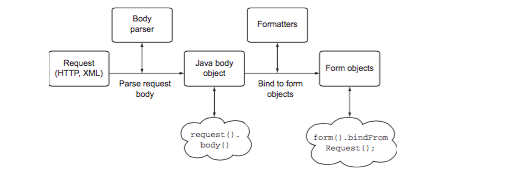
\includegraphics[scale=0.7]{Gambar/play-bodyparsers}
  \caption{Interaksi \textit{Body Parsers} dengan \textit{Request}} 
  \label{fig:2_play_bodyparsers}
\end{figure}

%\section{Kode KIRI (PHP)}
%\label{sec:kodeKIRI}


\textbf{Internationalization}\\
Pengguna aplikasi mungkin berasal dari beda negara dan bahasa, juga punya format yang berbeda untuk tanggal, angka, dan waktu. Kombinasi dari bahasa aturan format disebut \textit{locale}. Adaptasi program untuk berbeda \textit{locale} disebut \textit{internationalization (i18n)} atau \textit{localization (l10n)}. Perbedaan \textit{internationalization} dan \textit{localization} adalah \textit{internationalization} melakukan \textit{refactor} untuk menghapus kode lokal dari aplikasi, sedangkan \textit{localization} membuat versi lokal dari aplikasi. Program yang sudah diproses Internationalization mempunyai karakteristik:

\begin{itemize}
  \item Dengan penambahan data lokalisasi, eksekusi yang sama dapat dijalankan di seluruh dunia.
  \item Unsur tekstual, seperti pesan status dan komponen GUI, tidak ada \textit{hard-code} dalam program. Sebaliknya, pesan status dan komponen GUI disimpan di luar \textit{source code} dan diambil secara dinamis.
  \item Dengan adanya bahasa baru, program tidak perlu dikompilasi ulang.
  \item Data culturally-dependent, seperti tanggal dan mata uang, tampil dalam format yang sesuai dengan wilayah pengguna.
  \item Internationalization dapat dilakukan proses lokalisasi dengan cepat.
\end{itemize}

Untuk mendukung beberapa bahasa dalam Play, membuat kunci pesan yang dipetakan pesan sesungguhnya pada file pesan. Pesan ini dimuat dalam file messages.LANG dimana LANG merupakan bahasa yang dipakai. Messages.LANG disimpan dalam direktori conf. Sebagai contoh, terdapat dua bahasa yang dipakai pada aplikasi, yaitu Bahasa Inggris dan Bahasa Indonesia seperti pada kode listing \ref{lst_2_i18n_en} dan \ref{lst_2_i18n_id}

\begin{lstlisting}[caption=Contoh messages.en untuk i18n,label = {lst_2_i18n_en},language=Java]
  from = From:
  ph_from = e.g. Stasiun
  ph_to = e.g. Monas,Jakarta
  find = Find!
  to = To:
\end{lstlisting}

\begin{lstlisting}[caption=Contoh messages.id untuk i18n,label = {lst_2_i18n_id},language=Java]
  from = Dari:
  ph_from = misal: Stasiun
  ph_to = misal: Monas, Jakarta
  find = Cari!
  to = Ke:
\end{lstlisting}

Play harus mengetahui bahasa apa saja yang ada pada aplikasi sesuai dengan file messages.LANG. Untuk itu, daftarkan bahasa pada application.conf seperti pada kode listing \ref{lst_2_conf_i18n}. Pada \cite{playforjava}, konfigurasi bahasa dalam satu String. Tetapi pada Play Framework 2.4 konfigurasi bahasa dalam bentuk array of String.

\begin{lstlisting}[caption=Konfigurasi Bahasa i18n,label = {lst_2_conf_i18n},language=Java]
  ...
  # The application languages
  # ~~~~~
  play.i18n.langs = [ "en","id" ]
  ...
\end{lstlisting}

    \item Merancang dan mengimplementasikan kode KIRI yang sudah ada menjadi Play Framework.\\
    {\bf status :} Ada sejak rencana kerja skripsi.\\
    {\bf hasil :}    
    \begin{lstlisting}[caption=Template \textit{view} pada Play Framework]
@import play.i18n._
<!DOCTYPE html>


<html>

    <head>
        <title>KIRI</title>
        <link rel="shortcut icon" type="image/png" href="@routes.Assets.versioned("images/favicon.ico")">

        @*<link rel="stylesheet" href="@routes.Assets.versioned("openlayers/ol.css")" type="text/css">*@
        <link rel="stylesheet" href="@routes.Assets.versioned("foundation/css/foundation.min.css")" type="text/css">
        <link rel="stylesheet" href="@routes.Assets.versioned("css/styleIndex.css")" type="text/css">

        <script src="@routes.Assets.versioned("foundation/js/vendor/modernizr.js")"></script>

        <link rel="stylesheet" href="http://openlayers.org/en/v3.11.1/css/ol.css" type="text/css">
        <script src="http://openlayers.org/en/v3.11.1/build/ol.js" type="text/javascript"></script>
        @*<script src="@routes.Assets.versioned("openlayers/ol.js")"></script>*@
        @*<script src="http://openlayers.org/en/v3.10.1/build/ol.js" type="text/javascript"></script>*@

    </head>
    <body>
        @Messages.get("hello")
        <div class="row">

            <div id="controlpanel" class="large-3 large-push-9 columns">
                <div class="row center">
                    <img src="@routes.Assets.versioned("images/kiri200.png")" alt="KIRI logo" />
                </div>

                <div class="row">
                    <div class="small-5 columns">
                        <select class="fullwidth" id="regionselect">
                            <option value="bdg">Bandung</option>
                            <option value="jkt">Jakarta</option>
                            <option value="sby">Surabaya</option>
                            <option value="mlg">Malang</option>
                        </select>

                    </div>
                    <div class="small-7 columns">
                        <select class="fullwidth" id="localeselect">
                            <option value="en">English</option>
                            <option value="id">Bahasa Indonesia</option>
                        </select>
                    </div>
                </div>
                <div class="row">
                    <div class="small-2 columns">
                        <label for="startInput" class="inline">@Messages.get("from")</label>
                    </div>
                    <div class="small-10 columns">
                        <input type="text" id="startInput" value=""
                        placeholder="@Messages.get("ph_from")">
                    </div>
                </div>
                <div class="row">
                    <div class="large-12 columns">
                        <select id="startSelect" class="hidden"></select>
                    </div>
                </div>
                <div class="row">
                    <div class="small-2 columns">
                        <label for="finishInput" class="inline">@Messages.get("to")</label>
                    </div>
                    <div class="small-10 columns">
                        <input type="text" id="finishInput" value=""
                        placeholder="@Messages.get("ph_to")">
                    </div>
                </div>
                <div class="row">
                    <div class="large-12 columns">
                        <select id="finishSelect" class="hidden"></select>
                    </div>
                </div>
                <div class="row">
                    <div class="small-6 columns">
                        <a href="#" class="small button expand" id="findbutton"><strong>@Messages.get("find")</strong></a>
                    </div>
                    <div class="small-3 columns">
                        <a href="#" class="small button secondary expand" id="swapbutton">
                            <img src="@routes.Assets.versioned("images/swap.png")" alt="swap"/>
                        </a>
                    </div>
                    <div class="small-3 columns">
                        <a href="#" class="small button secondary expand" id="resetbutton">
                            <img src="@routes.Assets.versioned("images/reset.png")" alt="swap"/>
                        </a>
                    </div>
                </div>
                <div class="row">
                    <div class="large-12 columns" id="routingresults">
                        <div id="results-section-container"></div>
                    </div>
                </div>
                <div class="row">
                    <div class="large-12 columns">
                        <footer>
                            <a href="http://static.kiri.travel/$locale-apps">@Messages.get("apps")</a> |
                            <a href="http://classic.kiri.travel">@Messages.get("old")</a><br/>
                            <a href="http://static.kiri.travel/$locale-legal">@Messages.get("legal")</a> |
                            <a href="http://static.kiri.travel/$locale-feedback">@Messages.get("feedback")</a> |
                            <a href="http://static.kiri.travel/$locale-about">@Messages.get("about")</a>
                        </footer>
                            &nbsp;
                    </div>
                </div>
                <div class="row">
                </div>
            </div>

            <div id="map" class="large-9 large-pull-3 columns"></div>
        </div>


        <script src="@routes.Assets.versioned("foundation/js/vendor/jquery.js")"></script>
        <script src="@routes.Assets.versioned("foundation/js/vendor/fastclick.js")"></script>
        <script src="@routes.Assets.versioned("foundation/js/foundation.min.js")"></script>
        <script src="@routes.Assets.versioned("foundation/js/foundation/foundation.alert.js")"></script>

        <script src="@routes.Assets.versioned("js/newprotocol.js")"></script>
        <script src="@routes.Assets.versioned("js/index.js")"></script>


    </body>
</html>

    \end{lstlisting}
    
    

    \item Melakukan pengujian dan eksperimen.\\
    {\bf status :} Ada sejak rencana kerja skripsi.\\
    {\bf hasil :} 

    \item Membuat dokumen skripsi.\\
    {\bf status :} Ada sejak rencana kerja skripsi.\\
    {\bf hasil :} Dokumen skripsi sudah ditulis sampai dengan bab 3.

  \end{enumerate}

\bibliographystyle{ieeetr}
\bibliography{pustaka}

\section{Pencapaian Rencana Kerja}
Persentase penyelesaian skripsi sampai dengan dokumen ini dibuat dapat dilihat pada tabel berikut :

\begin{center}
  \begin{tabular}{ | c | c | c | c | l | c |}
    \hline
    1*  & 2*(\%) & 3*(\%) & 4*(\%) &5*(\%) & 6*(\%) \\ \hline \hline
    1   & 20  & 20  &  & & 15 \\ \hline
    2   & 20 & 20  &   & & 20\\ \hline
    3   & 20  &   & 20 & {\footnotesize Mengimplementasikan kode KIRI menjadi Play Framework} & 5 \\ \hline
    4   & 20  &   &  20 & {\footnotesize Pengujian seluruh fitur KIRI pada Play Framework} & \\ \hline
    5   & 20  & 10  & 10 & &10 \\ \hline
    Total  & 100  & 50  & 50 & & 50 \\ \hline
                          \end{tabular}
\end{center}

Keterangan (*)\\
1 : Bagian pengerjaan Skripsi (nomor disesuaikan dengan detail pengerjaan di bagian 5)\\
2 : Persentase total \\
3 : Persentase yang akan diselesaikan di Skripsi 1 \\
4 : Persentase yang akan diselesaikan di Skripsi 2 \\
5 : Penjelasan singkat apa yang dilakukan di S1 (Skripsi 1) atau S2 (skripsi 2)\\
6 : Persentase yang sudah diselesaikan sampai saat ini 

%\section{Kendala yang dihadapi}
%%TULISKAN BAGIAN INI JIKA DOKUMEN ANDA TIPE A ATAU C
%Kendala - kendala yang dihadapi selama mengerjakan skripsi :
%\begin{itemize}
%  \item Terlalu banyak melakukan prokratinasi
%  \item Terlalu banyak godaan berupa hiburan (game, film, dll)
%  \item Skripsi diambil bersamaan dengan kuliah ASD karena selama 5 semester pertama kuliah tersebut sangat dihindari dan tidak diambil, dan selama 4 semester terakhir kuliah tersebut selalu mendapat nilai E
%  \item Mengalami kesulitan pada saat sudah mulai membuat program komputer karena selama ini selalu dibantu teman
%\end{itemize}

\vspace{1cm}
\centering Bandung, \tanggal\\
\vspace{2cm} \nama \\ 
\vspace{1cm}

Menyetujui, \\
\ifdefstring{\jumpemb}{2}{
\vspace{1.5cm}
\begin{centering} Menyetujui,\\ \end{centering} \vspace{0.75cm}
\begin{minipage}[b]{0.45\linewidth}
% \centering Bandung, \makebox[0.5cm]{\hrulefill}/\makebox[0.5cm]{\hrulefill}/2013 \\
\vspace{2cm} Nama: \pembA \\ Pembimbing Utama
\end{minipage} \hspace{0.5cm}
\begin{minipage}[b]{0.45\linewidth}
% \centering Bandung, \makebox[0.5cm]{\hrulefill}/\makebox[0.5cm]{\hrulefill}/2013\\
\vspace{2cm} Nama: \pemB \\ Pembimbing Pendamping
\end{minipage}
\vspace{0.5cm}
}{
% \centering Bandung, \makebox[0.5cm]{\hrulefill}/\makebox[0.5cm]{\hrulefill}/2013\\
\vspace{2cm} Nama: \pembA \\ Pembimbing Tunggal
}
`
\end{document}

